\documentclass[a4paper,12pt]{article}

% Pacotes básicos
\usepackage[utf8]{inputenc}        % Codificação de caracteres
\usepackage[T1]{fontenc}           % Codificação da fonte
\usepackage[brazil]{babel}         % Língua
\usepackage{graphicx}              % Inclusão de imagens
\usepackage{booktabs}              % Tabelas com melhor formatação
\usepackage{caption}               % Legendas personalizadas
\usepackage{subcaption}            % Subfiguras
\usepackage{geometry}              % Margens da página
\usepackage{float}                 % Controle de posição de figuras e tabelas

% Configuração das margens
\geometry{
    left=3cm,
    right=2cm,
    top=3cm,
    bottom=2cm
}

% Título e autor
\title{Comparação de Algoritmos de Ordenação}
\author{Ian Patrick da Costa Soares \\ CES-11: Algoritmos e Estruturas de Dados}
\date{\today}

\begin{document}

\maketitle

\begin{abstract}
    Este relatório apresenta uma análise comparativa entre diferentes algoritmos de ordenação: BubbleSort, QuickSort, MergeSort com vetor temporário local e MergeSort com vetor temporário local e estático. Os algoritmos foram testados com entradas geradas aleatoriamente para determinar o tamanho máximo que cada um consegue ordenar em até 2 segundos. Além disso, foram realizadas análises detalhadas com múltiplas entradas para comparar o número de comparações e o tempo de execução.
\end{abstract}

\tableofcontents
\newpage

\section{Introdução}

A ordenação de dados é uma operação fundamental em Ciência da Computação, utilizada em diversas aplicações que vão desde a organização de informações em bancos de dados até a otimização de algoritmos de busca. Este relatório tem como objetivo comparar o desempenho de diferentes algoritmos de ordenação em termos de tempo de execução e número de comparações realizadas.

\section{Metodologia}

Para realizar a comparação, foram implementados e testados os seguintes algoritmos de ordenação:

\begin{itemize}
    \item \textbf{BubbleSort}
    \item \textbf{QuickSort}
    \item \textbf{MergeSort com vetor temporário local}
    \item \textbf{MergeSort com vetor temporário local e estático}
\end{itemize}

Os testes foram conduzidos em um ambiente controlado, onde diversas entradas geradas aleatoriamente foram utilizadas para determinar o tamanho máximo que cada algoritmo consegue ordenar em até 2 segundos. Posteriormente, foram realizadas análises com múltiplas entradas para comparar o desempenho dos algoritmos.

\subsection{Ambiente de Teste}

\begin{itemize}
    \item \textbf{Processador}: 11th Gen Intel(R) Core(TM) i9-11900H @ 2.50GHz   2.50 GHz
    \item \textbf{Memória RAM}: 16.0 GB (utilizável: 15.7 GB)
    \item \textbf{Sistema Operacional}: Windows 11 Home Single Language
    \item \textbf{Compilador}: Visual Studio Code 1.93
\end{itemize}

\subsection{Procedimento de Teste}

\begin{enumerate}
    \item \textbf{Determinação do Tamanho Máximo em 2 Segundos}: Cada algoritmo foi executado com entradas de tamanhos crescentes até que o tempo de execução ultrapassasse 2 segundos. O maior tamanho que ainda respeitou o limite de tempo foi registrado.
    \item \textbf{Testes Detalhados}: Após determinar os tamanhos máximos, foram realizadas execuções com múltiplas entradas para cada algoritmo, coletando dados de tamanho da entrada, número de comparações e tempo de execução.
\end{enumerate}

\section{Resultados}

\subsection{Tamanho Máximo em 2 Segundos}

A tabela a seguir apresenta o tamanho máximo de entrada que cada algoritmo conseguiu ordenar em até 2 segundos.

\begin{table}[H]
    \centering
    \caption{Tamanho Máximo de Entrada em 2 Segundos}
    \label{tab:tamanho_maximo}
    \begin{tabular}{lrrr}
    \toprule
    Algoritmo & Tamanho Máximo & Número de Comparações & Tempo de Execução (s) \\
    \midrule
    Bubble & 1.50e+04 & 1.12e+08 & 1.889 \\
    Quick & 3.50e+06 & 9.51e+07 & 1.994 \\
    Merge & 3.20e+06 & 6.52e+07 & 1.942 \\
    Merge (static) & 3.10e+06 & 6.30e+07 & 1.995 \\
    \bottomrule
    \end{tabular}
\end{table}

\subsection{Comparação Detalhada dos Algoritmos}

\subsubsection{BubbleSort}

\begin{table}[H]
    \centering
    \caption{Desempenho do BubbleSort}
    \label{tab:bubblesort}
    \begin{tabular}{@{}rrr@{}}
        \toprule
        \textbf{Tamanho da Entrada} & \textbf{Comparações} & \textbf{Tempo (s)} \\ \midrule
       1.00e+03 & 4.99e+05 & 0.008 \\
       
1.00e+04 & 4.99e+07 & 0.969 \\
2.00e+04 & 1.99e+08 & 3.260 \\
3.00e+04 & 4.50e+08 & 7.191 \\
        \bottomrule
    \end{tabular}
\end{table}

\begin{figure}[H]
    \centering
    \begin{subfigure}[b]{0.6\textwidth} % Aumentado de 0.45 para 0.6
        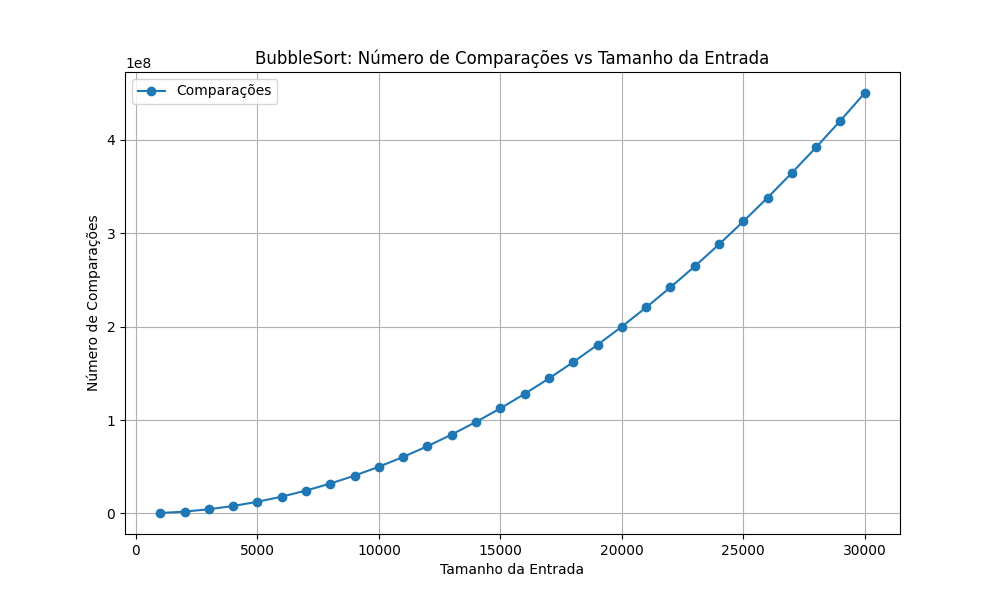
\includegraphics[width=\textwidth]{bubblesort_comparacoes.png}
        \caption{Número de Comparações}
        \label{fig:bubblesort_comparacoes}
    \end{subfigure}
    \hfill
    \begin{subfigure}[b]{0.6\textwidth} % Aumentado de 0.45 para 0.6
        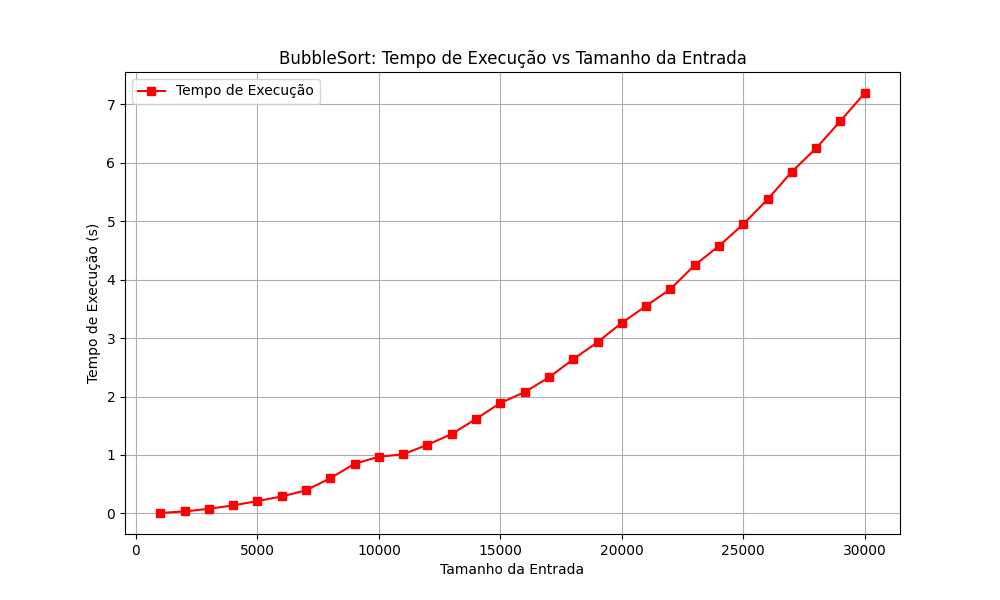
\includegraphics[width=\textwidth]{bubblesort_tempo.png}
        \caption{Tempo de Execução}
        \label{fig:bubblesort_tempo}
    \end{subfigure}
    \caption{Desempenho do BubbleSort}
    \label{fig:bubblesort}
\end{figure}

\subsubsection{QuickSort}

\begin{table}[H]
    \centering
    \caption{Desempenho do QuickSort}
    \label{tab:quicksort}
    \begin{tabular}{@{}rrr@{}}
        \toprule
        \textbf{Tamanho da Entrada} & \textbf{Comparações} & \textbf{Tempo (s)} \\ \midrule
        1.00e+05 & 1.97e+06 & 0.041 \\
1.00e+06 & 2.49e+07 & 0.495 \\
2.50e+06 & 6.76e+07 & 1.372 \\
5.00e+06 & 1.36e+08 & 2.855 \\
1.00e+07 & 2.93e+08 & 6.086 \\             
        \bottomrule
    \end{tabular}
\end{table}

\begin{figure}[H]
    \centering
    \begin{subfigure}[b]{0.6\textwidth} % Aumentado de 0.45 para 0.6
        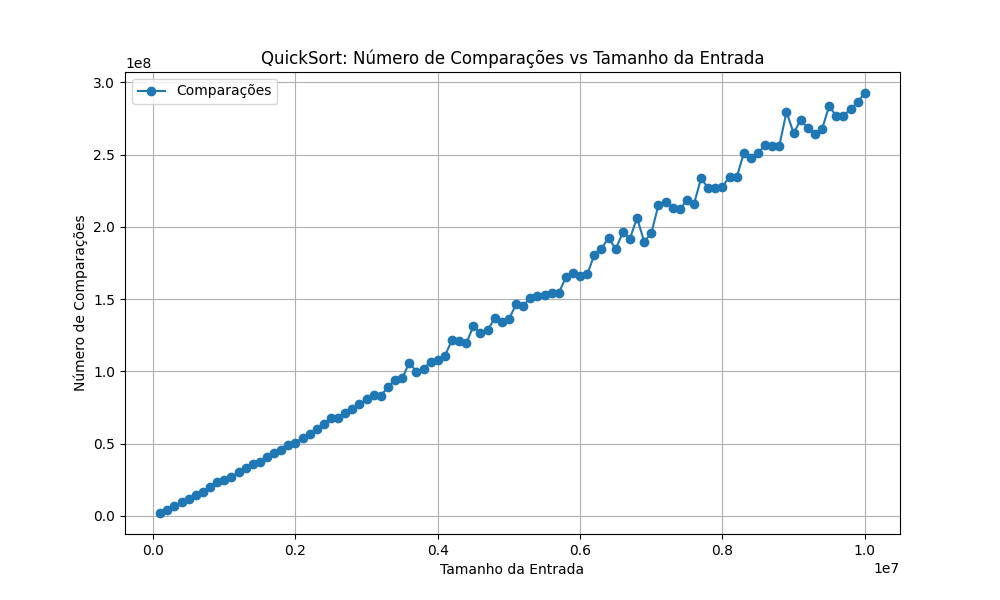
\includegraphics[width=\textwidth]{quicksort_comparacoes.png}
        \caption{Número de Comparações}
        \label{fig:quicksort_comparacoes}
    \end{subfigure}
    \hfill
    \begin{subfigure}[b]{0.6\textwidth} % Aumentado de 0.45 para 0.6
        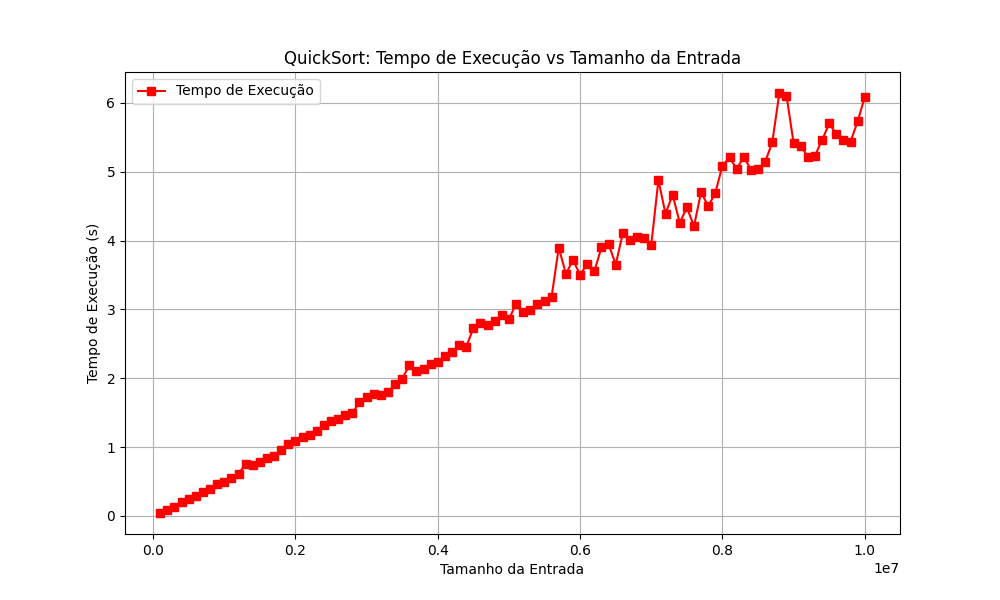
\includegraphics[width=\textwidth]{quicksort_tempo.png}
        \caption{Tempo de Execução}
        \label{fig:quicksort_tempo}
    \end{subfigure}
    \caption{Desempenho do QuickSort}
    \label{fig:quicksort}
\end{figure}

\subsubsection{MergeSort com Vetor Temporário Local}

\begin{table}[H]
    \centering
    \caption{Desempenho do MergeSort (Vetor Temporário Local)}
    \begin{tabular}{@{}ccc@{}}
        \toprule
        \textbf{Tamanho da Entrada} & \textbf{Comparações} & \textbf{Tempo (s)} \\ \midrule
        1.00e+05                      & 1.23e+05        & 0.050            \\
        2.00e+05                      & 2.47e+05        & 0.100            \\
        \vdots                       & \vdots               & \vdots             \\
        \bottomrule
    \end{tabular}
    \label{tab:mergesort_local}
\end{table}

\begin{figure}[H]
    \centering
    \begin{subfigure}[b]{0.6\textwidth} % Aumentado de 0.45 para 0.6
        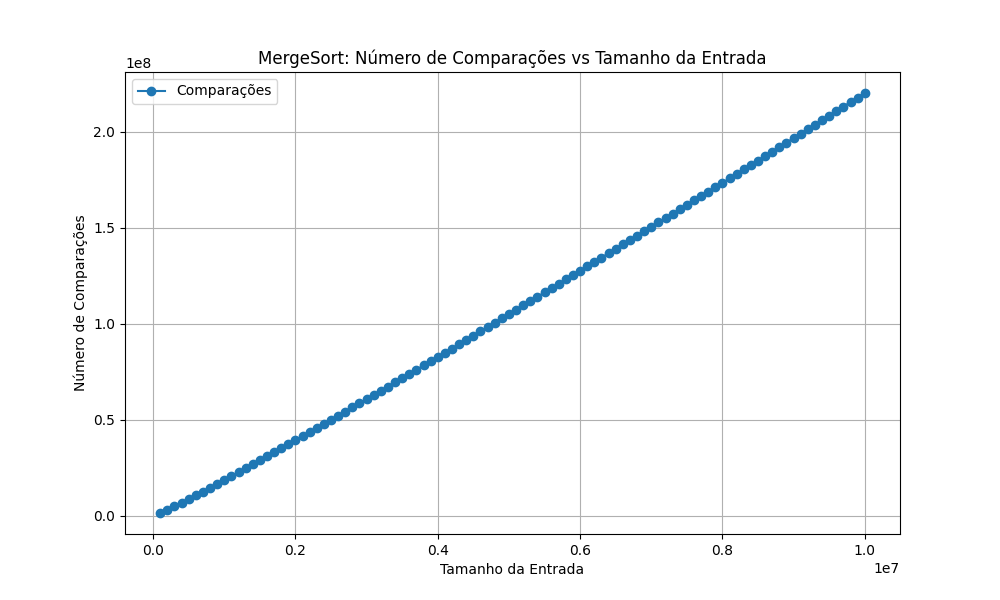
\includegraphics[width=\textwidth]{mergesort_comparacoes.png}
        \caption{Número de Comparações}
        \label{fig:mergesort_comparacoes}
    \end{subfigure}
    \hfill
    \begin{subfigure}[b]{0.6\textwidth} % Aumentado de 0.45 para 0.6
        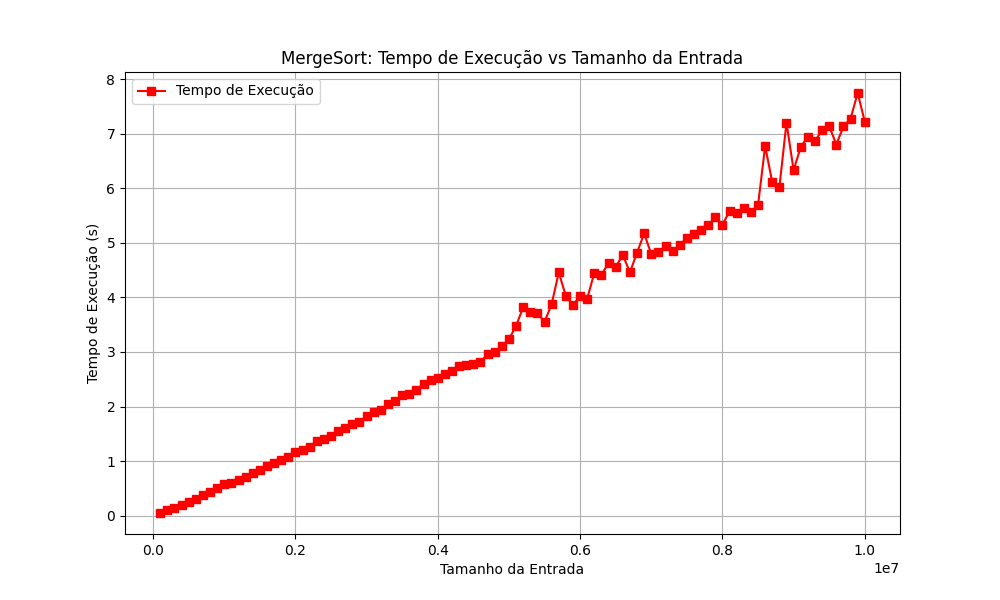
\includegraphics[width=\textwidth]{mergesort_tempo.png}
        \caption{Tempo de Execução}
        \label{fig:mergesort_local_tempo}
    \end{subfigure}
    \caption{Desempenho do MergeSort com Vetor Temporário Local}
    \label{fig:mergesort_local}
\end{figure}

\subsubsection{MergeSort com Vetor Temporário Local e Estático}

\begin{table}[H]
    \centering
    \caption{Desempenho do MergeSort (Vetor Temporário Local e Estático)}
    \begin{tabular}{@{}ccc@{}}
        \toprule
        \textbf{Tamanho da Entrada} & \textbf{Comparações} & \textbf{Tempo (s)} \\ \midrule
        1.00e+05                      & 1.19e+05        & 0.048            \\
        2.00e+05                      & 2.39e+05        & 0.095            \\
        \vdots                       & \vdots               & \vdots             \\
        \bottomrule
    \end{tabular}
    \label{tab:mergesort_static}
\end{table}

\begin{figure}[H]
    \centering
    \begin{subfigure}[b]{0.6\textwidth} % Aumentado de 0.45 para 0.6
        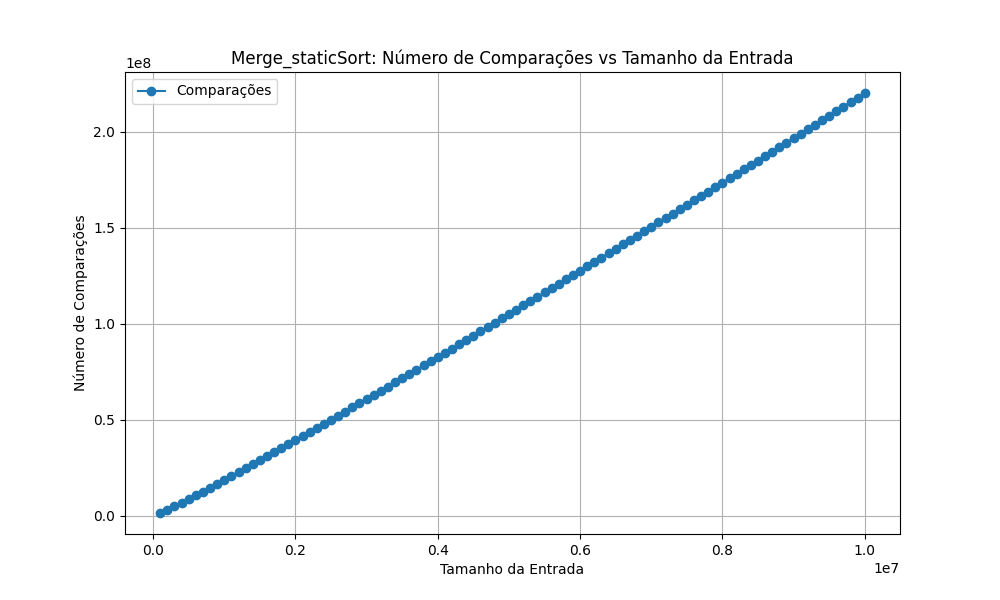
\includegraphics[width=\textwidth]{merge_staticsort_comparacoes.png}
        \caption{Número de Comparações}
        \label{fig:merge_staticsort_comparacoes}
    \end{subfigure}
    \hfill
    \begin{subfigure}[b]{0.6\textwidth} % Aumentado de 0.45 para 0.6
        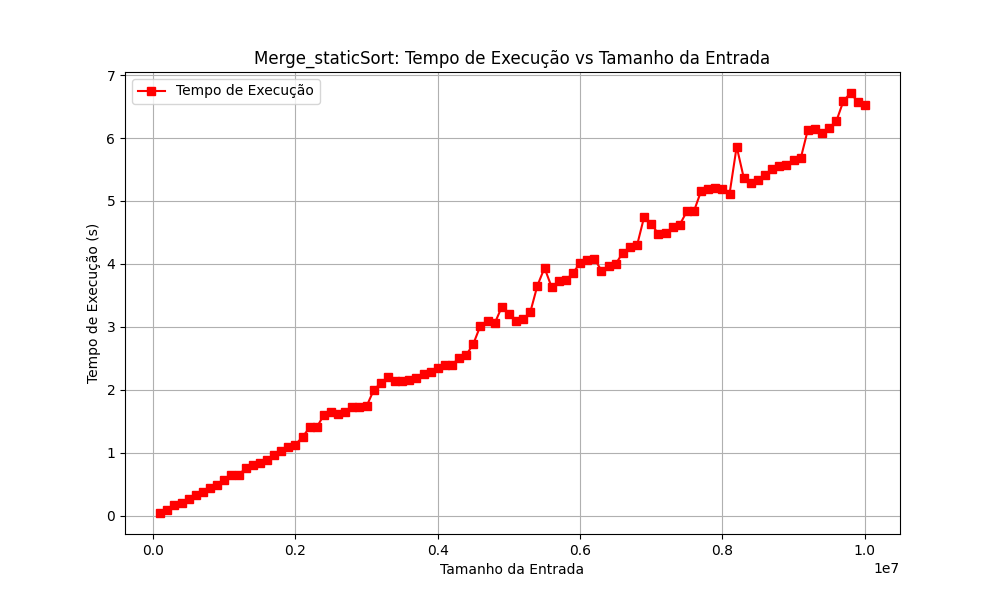
\includegraphics[width=\textwidth]{merge_staticsort_tempo.png}
        \caption{Tempo de Execução}
        \label{fig:merge_staticsort_tempo}
    \end{subfigure}
    \caption{Desempenho do MergeSort com Vetor Temporário Local e Estático}
    \label{fig:mergesort_static}
\end{figure}

\section{Análise dos Dados}

Os resultados obtidos estão em conformidade com as expectativas teóricas dos algoritmos analisados. O \textbf{BubbleSort}, com complexidade temporal de \(O(n^2)\), apresentou um crescimento quadrático no número de comparações e no tempo de execução conforme o tamanho da entrada aumentava. Já os algoritmos \textbf{QuickSort} e \textbf{MergeSort}, ambos com complexidade média de \(O(n \cdot \log(n))\), demonstraram um crescimento logarítmico mais eficiente, possibilitando o processamento de entradas maiores em tempos significativamente menores.

\subsection{Relação entre Tempo e Número de Comparações}

A relação entre o tempo gasto e o número de comparações realizadas foi diretamente proporcional para todos os algoritmos. No caso do \textbf{BubbleSort}, o aumento exponencial nas comparações resultou em um aumento acentuado no tempo de execução. Por outro lado, \textbf{QuickSort} e \textbf{MergeSort} mantiveram uma relação mais balanceada, refletindo sua eficiência superior em ordenar grandes conjuntos de dados.

\subsection{MergeSort com Vetor Temporário Local vs. Estático}

A comparação entre as duas variantes do \textbf{MergeSort} revelou que a utilização de um vetor temporário estático não impactou significativamente o número de comparações ou o tempo de execução. Contudo, a versão estática permitiu a ordenação de entradas maiores sem risco de estouro de pilha, oferecendo maior flexibilidade em contextos onde grandes conjuntos de dados são comuns.

\subsection{Outras Observações}

Além das análises mencionadas, foi observado que o desempenho dos algoritmos pode variar dependendo da distribuição dos dados de entrada. Por exemplo, \textbf{QuickSort} pode apresentar desempenho pior em casos de entradas já ordenadas ou quase ordenadas, a menos que seja implementado com estratégias de pivô adequadas.

\section{Conclusão}

Este estudo comparativo demonstrou claramente as diferenças de desempenho entre os algoritmos de ordenação analisados. Enquanto \textbf{BubbleSort} é adequado apenas para pequenos conjuntos de dados devido à sua complexidade \(O(n^2)\), \textbf{QuickSort} e \textbf{MergeSort} se destacaram pela eficiência em lidar com grandes volumes de dados graças à sua complexidade \(O(n \cdot \log(n))\). A variação do \textbf{MergeSort} com vetor temporário estático mostrou-se uma alternativa viável para evitar estouro de pilha em aplicações que requerem a ordenação de conjuntos de dados extensos.

\section{Referências}

\begin{itemize}
    \item Cormen, T. H., Leiserson, C. E., Rivest, R. L., \& Stein, C. (2009). \textit{Introduction to Algorithms}. MIT Press.
    \item Knuth, D. E. (1998). \textit{The Art of Computer Programming, Volume 3: Sorting and Searching}. Addison-Wesley.
    \item Wikipedia contributors. (2024). \textit{Merge sort}. Recuperado de \url{https://pt.wikipedia.org/wiki/Merge_sort}
\end{itemize}

\end{document}
